%%%%%%%%%%%%%%%%%%%%%%%%%%%%%%%%%%%%%%%%%
% Make sure to set your name, legi number and url to the right git branch.
\newcommand{\hmwkAuthorName}{Yu-chen Tsai} % Your name
\newcommand{\hmwkAuthorLegi}{16-929-747} % Your name
\newcommand{\hmwkGitBranch}{16-929-747/1 locally linear embedding} % Your name
%
%%%%%%%%%%%%%%%%%%%%%%%%%%%%%%%%%%%%%%%%%

%----------------------------------------------------------------------------------------
%	PACKAGES AND OTHER DOCUMENT CONFIGURATIONS
%	Skip this
%----------------------------------------------------------------------------------------

\documentclass{article}

\usepackage{fancyhdr} % Required for custom headers
\usepackage{lastpage} % Required to determine the last page for the footer
\usepackage{extramarks} % Required for headers and footers
\usepackage{graphicx} % Required to insert images
\usepackage{lipsum} % Used for inserting dummy 'Lorem ipsum' text into the template

% Margins
\topmargin=-0.45in
\evensidemargin=0in
\oddsidemargin=0in
\textwidth=6.5in
\textheight=9.0in
\headsep=0.25in 

\linespread{1.1} % Line spacing

% Set up the header and footer
\pagestyle{fancy}
\lhead{\hmwkAuthorName} % Top left header
\chead{\hmwkClass\ \hmwkTitle} % Top center header
\rhead{\firstxmark} % Top right header
\lfoot{\lastxmark} % Bottom left footer
\cfoot{} % Bottom center footer
\rfoot{Page\ \thepage\ of\ \pageref{LastPage}} % Bottom right footer
\renewcommand\headrulewidth{0.4pt} % Size of the header rule
\renewcommand\footrulewidth{0.4pt} % Size of the footer rule

\setlength\parindent{0pt} % Removes all indentation from paragraphs

%----------------------------------------------------------------------------------------
%	DOCUMENT STRUCTURE COMMANDS
%	Skip this
%----------------------------------------------------------------------------------------

% Header and footer for when a page split occurs within a problem environment
\newcommand{\enterProblemHeader}[1]{
\nobreak\extramarks{#1}{#1 continued on next page\ldots}\nobreak
\nobreak\extramarks{#1 (continued)}{#1 continued on next page\ldots}\nobreak
}

% Header and footer for when a page split occurs between problem environments
\newcommand{\exitProblemHeader}[1]{
\nobreak\extramarks{#1 (continued)}{#1 continued on next page\ldots}\nobreak
\nobreak\extramarks{#1}{}\nobreak
}

\setcounter{secnumdepth}{0} % Removes default section numbers
\newcounter{homeworkProblemCounter} % Creates a counter to keep track of the number of problems

\newcommand{\homeworkProblemName}{}
\newenvironment{homeworkProblem}[1][Problem \arabic{homeworkProblemCounter}]{ % Makes a new environment called homeworkProblem which takes 1 argument (custom name) but the default is "Problem #"
\stepcounter{homeworkProblemCounter} % Increase counter for number of problems
\renewcommand{\homeworkProblemName}{#1} % Assign \homeworkProblemName the name of the problem
\section{\homeworkProblemName} % Make a section in the document with the custom problem count
\enterProblemHeader{\homeworkProblemName} % Header and footer within the environment
}{
\exitProblemHeader{\homeworkProblemName} % Header and footer after the environment
}

\newcommand{\problemAnswer}[1]{ % Defines the problem answer command with the content as the only argument
\noindent\framebox[\columnwidth][c]{\begin{minipage}{0.98\columnwidth}#1\end{minipage}} % Makes the box around the problem answer and puts the content inside
}

\newcommand{\homeworkSectionName}{}
\newenvironment{homeworkSection}[1]{ % New environment for sections within homework problems, takes 1 argument - the name of the section
\renewcommand{\homeworkSectionName}{#1} % Assign \homeworkSectionName to the name of the section from the environment argument
\subsection{\homeworkSectionName} % Make a subsection with the custom name of the subsection
\enterProblemHeader{\homeworkProblemName\ [\homeworkSectionName]} % Header and footer within the environment
}{
\enterProblemHeader{\homeworkProblemName} % Header and footer after the environment
}
   
%----------------------------------------------------------------------------------------
%	NAME AND CLASS SECTION
%	Skip this
%----------------------------------------------------------------------------------------

\newcommand{\hmwkTitle}{Locally Linear Embedding} % Assignment title
\newcommand{\hmwkDueDate}{Monday,\ March\ 6th,\ 2017} % Due date
\newcommand{\hmwkClass}{SLT coding exercise\ \#1} % Course/class
\newcommand{\hmwkClassTime}{Mo 16:15} % Class/lecture time
\newcommand{\hmwkClassInstructor}{} % Teacher/lecturer

%----------------------------------------------------------------------------------------
%	TITLE PAGE
%	Skip this
%----------------------------------------------------------------------------------------

\title{
\vspace{2in}
\textmd{\small{\hmwkClass}}\\
\textmd{\textbf{\hmwkTitle}}\\
\small{https://gitlab.vis.ethz.ch/vwegmayr/slt-coding-exercises}\\
\normalsize\vspace{0.1in}\small{Due\ on\ \hmwkDueDate}
%\vspace{0.1in}\large{\textit{\hmwkClassInstructor\ \hmwkClassTime}}
\vspace{3in}
}

\author{
\hmwkAuthorName\\
\hmwkAuthorLegi
}

\date{ } % Insert date here if you want it to appear below your name

\begin{document}

\maketitle

%----------------------------------------------------------------------------------------
%	TABLE OF CONTENTS
%	Skip this
%----------------------------------------------------------------------------------------

%\setcounter{tocdepth}{1} % Uncomment this line if you don't want subsections listed in the ToC

\newpage
\tableofcontents
\newpage

%----------------------------------------------------------------------------------------
%	SECTIONS
%	Now you are in the right hood
%----------------------------------------------------------------------------------------

\begin{homeworkProblem}[The Model]
The model section is intended to allow you to recapitulate the essential ingredients used in \hmwkTitle. Write down the \textit{necessary} equations to specify \hmwkTitle\ and and shortly explain the variables that are involved. This section should only introduce the equations, their solution should be outlined in the implementation section.\newline
Hard limit: One page
\vspace{10pt}

\problemAnswer{ % Answer
Your Answer
$$\mathcal{E}(W)=\sum_i{|\vec{X_i}-\sum_j{W_{ij}\vec{X_j}}|^2}$$
$$\sum_j{W_{ij}}=1$$
$$\Phi(Y)=\sum_i{|\vec{Y_i}-\sum_j{W_{ij}\vec{Y_j}}|^2}$$
$$\sum_i{\vec{Y_i}}=0$$
$$\frac{1}{N}\sum_i{\vec{Y_i}\vec{Y_i}^T}=I$$

\begin{enumerate}
    \item 
    For each $\vec{X_i}$, one identifies the neighbors $\vec{X_j}$ of it either by K nearest points in Euclidean distance or other sophisticated rules based on local metrics.
    \item
    Because the reconstruction error should be invariant to translation, the rows of the weight matrix $W$ have to sum to one.
    \item
    The cost function of the mapping is defined as sum of the reconstruction error of mapped vectors.
    \item
    The embedding should be invariant of translation and scaling, so one can remove two degrees of freedom by making $Y$ has zero mean and unit variance. 
\end{enumerate}
}
\end{homeworkProblem}
\clearpage

%----------------------------------------------------------------------------------------
\begin{homeworkProblem}[The Questions]
This is the core section of your report, which contains the tasks for this exercise and your respective solutions. Make sure you present your results in an illustrative way by making use of graphics, plots, tables, etc. so that a reader can understand the results with a single glance. Check that your graphics have enough resolution or are vector graphics. Consider the use of GIFs when appropriate.\newline
Hard limit: Two pages

\begin{homeworkSection}{(a) Get the data}
For this exercise we will work with the MNIST data set. In order to learn more about it and download it, go to http://yann.lecun.com/exdb/mnist/.
\end{homeworkSection}

\begin{homeworkSection}{(b) Locally linear embedding}
Implement the LLE algorithm and apply it to the MNIST data set. Provide descriptive visualizations for 2D \& 3D embedding spaces. Is it possible to see clusters?
\end{homeworkSection}

\begin{homeworkSection}{(c) Cluster structure}
Investigate the cluster structure of the data. Can you observe block structures in the $M$ matrix (use matrix plots)? Also plot the singular values of $M$. Do you notice something?
Can you think of ways to determine the optimal embedding dimension?
\end{homeworkSection}

\begin{homeworkSection}{(d) Nearest Neighbors}
Investigate the influence of the choice of how many nearest neighbors you take into account. Additionally, try different metrics to find the nearest neighbors (we are dealing with images!).
\end{homeworkSection}

\begin{homeworkSection}{(e) Linear manifold interpolation}
Assume you pick some point in the embedding space. How can you map it back to the original (high dimensional) space? Investigate how well this works for points within and outside the manifold (does it depend on the dimensionality of the embedding space?) Try things like linearly interpolating between two embedding vectors and plot the sequence of images along that line. What happens if you do that in the original space?
\end{homeworkSection}

\vspace{10pt}
\problemAnswer{ % Answer
\begin{homeworkSection}{(b) Locally linear embedding}
\end{homeworkSection}

Yes, as the number of neighbors used for computing the embedding increases, we can see it gets easier to separate the clusters of different digits. And it is worth to mention that, as one can see, the 2 dimensional embedding is actually a projection of the 3 dimensional embedding. 
\newline \newline
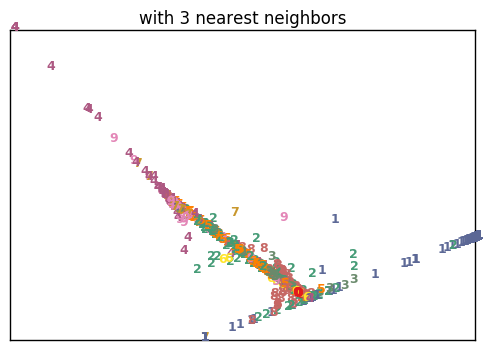
\includegraphics[scale=0.428]{./pic/n_1000_k_3.png} 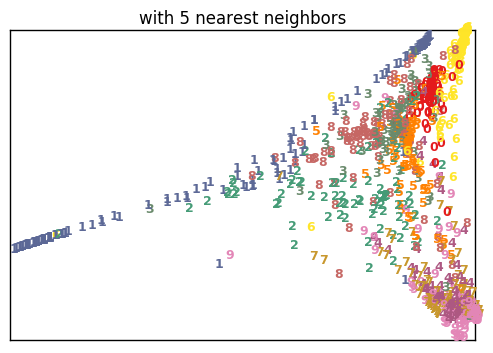
\includegraphics[scale=0.428]{./pic/n_1000_k_5.png} 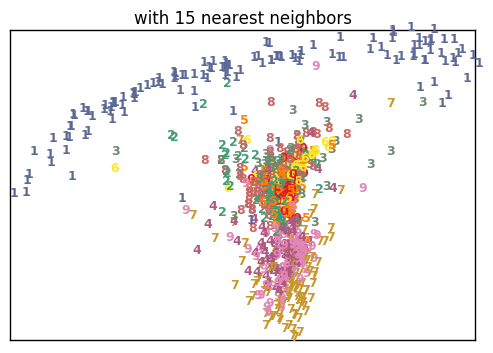
\includegraphics[scale=0.428]{./pic/n_1000_k_15.png}


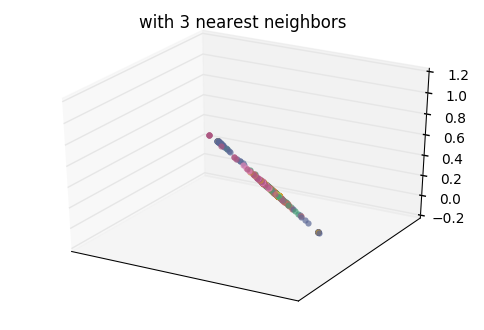
\includegraphics[scale=0.428]{./pic/n_1000_k_3_3d.png} 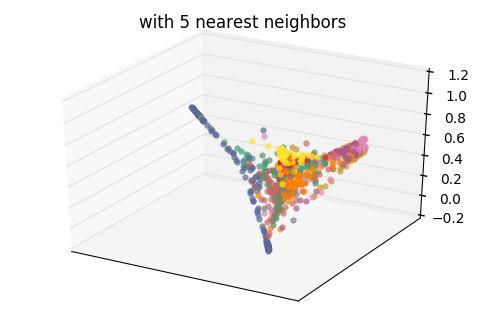
\includegraphics[scale=0.428]{./pic/n_1000_k_5_3d.png} 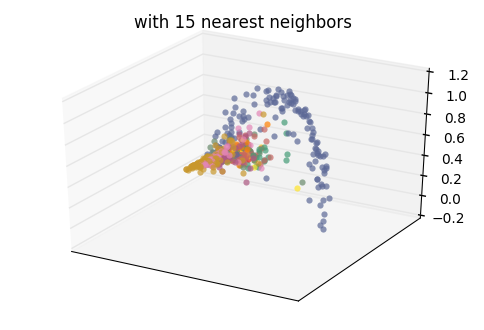
\includegraphics[scale=0.428]{./pic/n_1000_k_15_3d.png}

\begin{homeworkSection}{(c) Cluster structure}
\end{homeworkSection}
\begin{center}
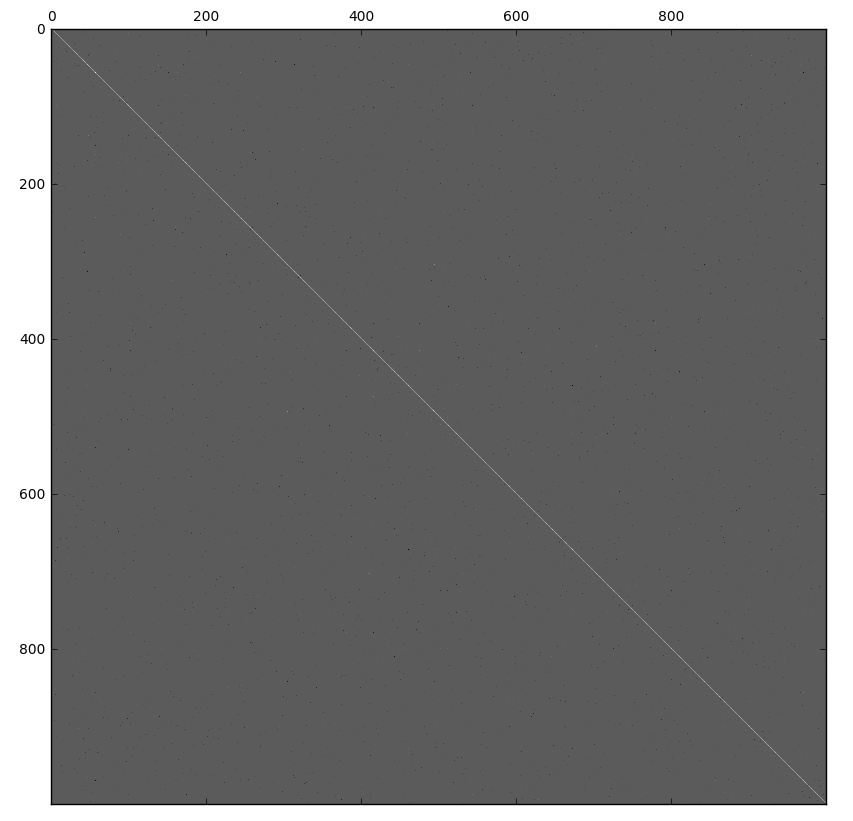
\includegraphics[scale=0.3]{./pic/M.png}\\
Matrix plot of M\\
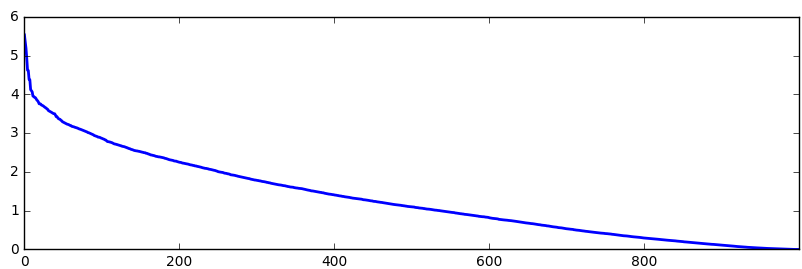
\includegraphics[scale=0.3]{./pic/M_eigenvalue.png}\\
Eigenvalues of M (sorted)\\
\end{center}
Honestly, I didn't observe any "block" structures in the matrix plot. But I think it depends on the dataset. If the space of the data can be partitioned  into m subspace, then maybe we can observe m blocks on the diagonal of the matrix plot indicating that the problem can be divided into smaller embedding problems. 
}
\end{homeworkProblem}
\clearpage

\vspace{10pt}
\problemAnswer{ % Answer
One can observe that there is a turning point in the growth of eigenvalues.
Because the value of the cost function $\Phi(Y)$ is actually the sum of smallest d + 1 eigenvalues (including at least one zero), we can determine the embedding dimension by observing the growth of eigenvalues(sorted from lowest to highest) and then pick a d that is smaller than the point where eigenvalue starts to grow rapidly.
\begin{homeworkSection}{(d) Nearest Neighbors}
\end{homeworkSection}
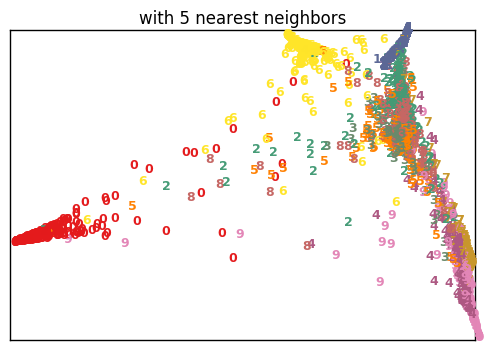
\includegraphics[scale=0.428]{./pic/n_2000_k_5.png}
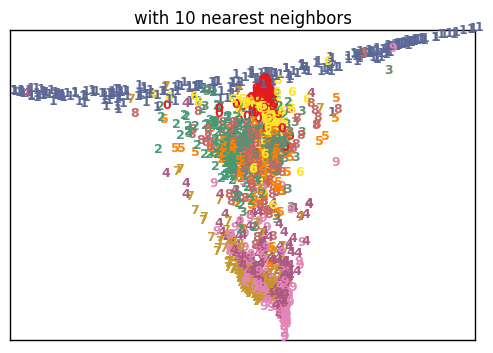
\includegraphics[scale=0.428]{./pic/n_2000_k_10.png}
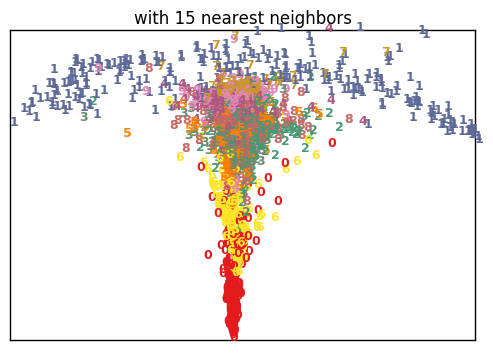
\includegraphics[scale=0.428]{./pic/n_2000_k_15.png}
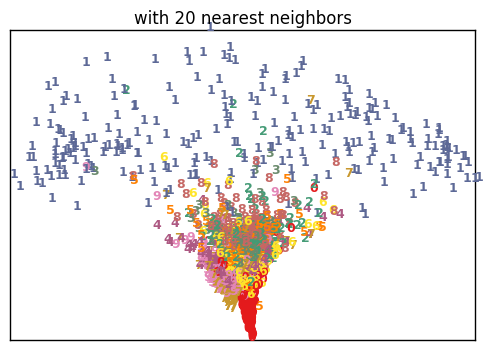
\includegraphics[scale=0.428]{./pic/n_2000_k_20.png}
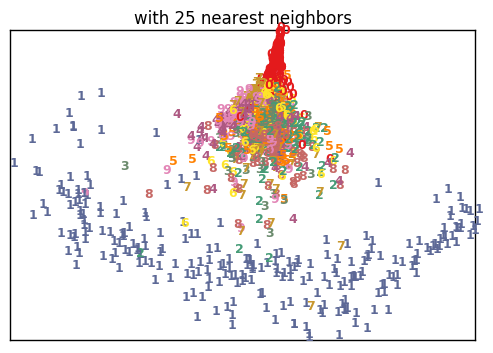
\includegraphics[scale=0.428]{./pic/n_2000_k_25.png}
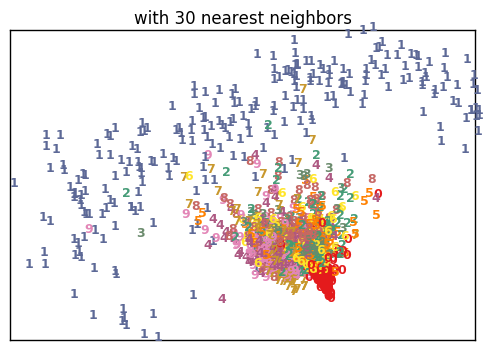
\includegraphics[scale=0.428]{./pic/n_2000_k_30.png}\\
We can see that increasing the number of neighbors from 5 to 15 does make the clusters of each digit easier to separate, but more than 15 neighbors doesn't improve the result a lot. Maybe it's because the number of points I used here is 2000, so when we consider too many neighbors, we may include points of different digits. And this will only hinder the embedding algorithm to find a good embedding where digits are visually separated. \\\\
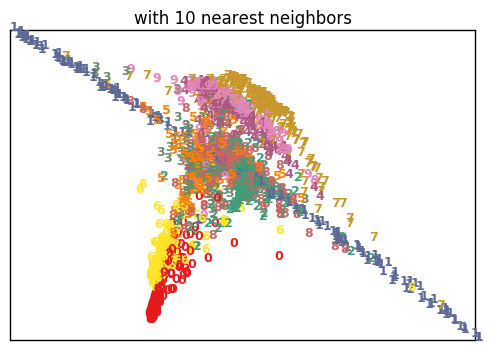
\includegraphics[scale=0.65]{./pic/n_2000_k_10_compare.png}
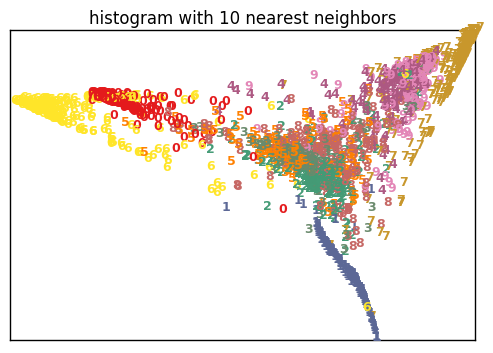
\includegraphics[scale=0.65]{./pic/n_2000_k_10_compare_hist.png}


Because we are dealing with images here, it might helps to use histogram of sliding windows instead of raw image. Here I tried to compute the 8-bin histogram of 7x7 sliding window of step size 3, and concatenated them together as our new feature vector. In total it has 1352 dimensions. As we can see in the figures above, using histogram really improve the embedding result. Windows of proper size and step size can keep the important information and ignore the noise, that's why the result is better.
}
\clearpage


\vspace{10pt}
\problemAnswer{ % Answer
\begin{homeworkSection}{(e) Linear manifold interpolation}

Given a point $y_i$ in the embedding space, we first find the nearest neighbors of it in the embedding space, and computer the weights $w_j$ of them by
$$w_j=\frac{\sum_k{C_{jk}^{-1}}}{\sum_{lk}{C_{lk}^{-1}}}$$
where $C_{jk}=(y_i-y_j)^T(y_i-y_k)$. And then, construct $x_i$ in the original space by 
$$x_i=\sum_j{w_jx_j}$$

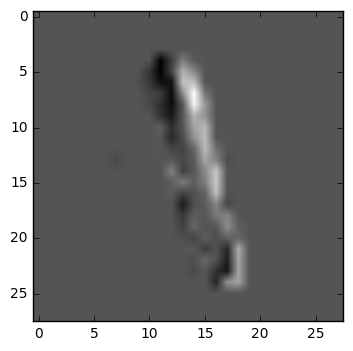
\includegraphics[scale=0.88]{./pic/recover_1_0.png}
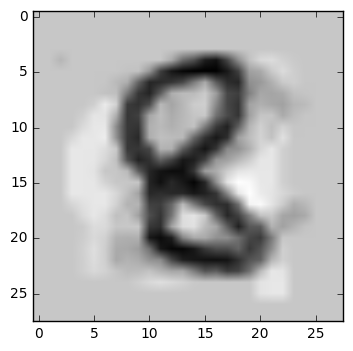
\includegraphics[scale=0.88]{./pic/recover_0_0.png}\\
The left figure is a combination of neighbors of digit 1, the right figure is a combination of digit 2,3,8, and 9. The problem of this method is clear: when the picked point is in the embedding space but outside the manifold, the nearest neighbors are likely come from different clusters(because they are all far away). And the corresponding reconstruction may be totally meaningless.

\end{homeworkSection}

}
\clearpage
%----------------------------------------------------------------------------------------
\begin{homeworkProblem}[The Implementation]
In the implementation section you give a concise insight to the practical aspects of this coding exercise. It mainly mentions the optimization methods used to solve the model equations. Did you encounter numerical or efficiency problems? If yes, how did you solve them?
Provide the link to your git branch of this coding exercise.\newline
Hard limit: One page

\vspace{10pt}
\problemAnswer{ % Answer
\begin{enumerate}
    \item 
    Sometimes $C$ is singular or nearly singular, the program report error message at the matrix inversion step. And this typically arises when $K$ is large. One way to avoid the numerical difficulty is adding small values on all the diagonal terms of C as regularization.
    \item
    All the calculations have closed form solution, so no optimization used to solve the equations. The only mathematical libraries used is the inverse matrix solver and eigenvalue decomposition solver in numpy.
    \item
    Because of the limit of memory and time, all the experiments only run on less than 2000 points randomly selected from the original 70000 points.
\end{enumerate}
}
\end{homeworkProblem}
\clearpage

%----------------------------------------------------------------------------------------
\begin{homeworkProblem}[Your Page]
Your page gives you space to include ideas, observations and results which do not fall into the categories provided by us. You can also use it as an appendix to include things which did not have space in the other sections.\newline
No page limit.

\vspace{10pt}
\problemAnswer{ % Answer
Your Answer

\hmwkGitBranch % defined in line 5
}
\end{homeworkProblem}
\clearpage

\end{document}

